\chapter{Desarrollo del \emph{framework}}

En este capitulo, trataremos los asuntos concernientes a la construcción de las
funciones del \emph{framework}, sobre las que recaen la automatización de los
casos de prueba, y la expansibilidad que pueda darse a todo el proyecto.

Si bien en el anterior capitulo el tema fundamental era el análisis y
exploración que se realizo sobre el software, el objeto central de este
capitulo es el \emph{framework} mismo.

\section{Estructura del \emph{framework}}
El \emph{framework} desarrollado basa su estructura y comportamiento en las
recomendaciones de la biblioteca utilizada (\emph{webdriver.io}), esta puede
verse en la \emph{figura \ref{estructura}}.

\begin{figure}
\centering
\begin{tikzpicture}[
    grow via three points={one child at (0.5,-0.7) and
    two children at (0.5,-0.7) and (0.5,-1.4)},
    edge from parent path={(\tikzparentnode.south) |- (\tikzchildnode.west)}]
    \node {salesforce\_automation}
        child { node {Errors}}
        child { node {PageObjects}
            child { node {New}
                child { node {ListView.po.js}}
                child { node {PriceBook.po.js}}
                child { node {Product.po.js}}
            }
            child [missing] {}
            child [missing] {}
            child [missing] {}
            child { node {Card.po.js}}
            child { node {Confirmation.po.js}}
            child { node {Launcher.po.js}}
            child { node {List.po.js}}
            child { node {Login.po.js}}
            child { node {Message.po.js}}
            child { node {Modal.po.js}}
            child { node {Profile.po.js}}
            child { node {Row.po.js}}
            child { node {Setup.po.js}}
            child { node {View.po.js}}
        }
        child [missing] {}
        child [missing] {}
        child [missing] {}
        child [missing] {}
        child [missing] {}
        child [missing] {}
        child [missing] {}
        child [missing] {}
        child [missing] {}
        child [missing] {}
        child [missing] {}
        child [missing] {}
        child [missing] {}
        child [missing] {}
        child [missing] {}
        child { node {Specs}
            child { node {001.F001.js}}
            child { node {002.F002.js}}
            child { node {003.A001.js}}
            child { node {\ldots.js}}
        }
        child [missing] {}
        child [missing] {}
        child [missing] {}
        child [missing] {}
        child { node {Utils}
            child { node {Common.js}}
        }
        child [missing] {}
        child { node {config.js}}
        child { node {package.json}}
        child { node {wdio.conf.js}};
\end{tikzpicture}
\caption{Estructura de archivos del \emph{framework}.}
\label{estructura}
\source{Elaboración propia.}
\end{figure}

Puede observarse en esta figura, que se creó la carpeta \textbf{PageObjects}
para albergar todas las clases que representan elementos de las paginas que
componen el \emph{framework}, además de una carpeta \textbf{Specs} que alberga
los casos de prueba automatizados, adicionalmente existe la carpeta
\textbf{Utils} donde se ubicaron funciones adicionales utilitarias.

Adicionalmente a estas carpetas también se encuentran los ficheros relacionados
con la biblioteca \emph{webdriver.io}, utilizados como se detallan a
continuación:

\begin{description}
    \item [\emph{config.dist.js}] Archivo de configuración del \emph{framework},
    sin credenciales para ser versionado con el sistema de control de cambios.
\item [\emph{config.js}] Archivo de configuración del \emph{framework}, donde
    están parametrizados todas las variables y credenciales necesarias durante
    la ejecución.
\item [\emph{docker-compose.yml}] Archivo de orquestación de imágenes utilizados
    para la ejecución de los casos de prueba sobre imágenes de \emph{Docker}.
\item [\emph{package.json}] Archivo de configuración de \emph{node.js}, que
    incluye los diferentes tipos de ejecución disponible, las bibliotecas
    utilizadas, entre otros detalles menores acerca del proyecto.
\item [\emph{wdio.browserstack.conf.js}] Archivo de configuración utilizado por
    la biblioteca \emph{webdriver.io} para la ejecución de las pruebas sobre el
    servicio \emph{BrowserStack}.
\item [\emph{wdio.conf.js}] Archivo de configuración de \emph{webdriver.io},
    este contiene las conjuntos de pruebas disponibles, entre otras variables
    utilizadas por el entorno de prueba.
\item [\emph{wdio.docker.conf.js}] Archivo de configuración utilizado por la
    biblioteca \emph{webdriver.io} para la ejecución de las pruebas sobre el
    servidor \emph{Docker}.
\item [\emph{wdio.standalone.conf.js}] Archivo de configuración utilizado por la
    biblioteca \emph{webdriver.io} para la ejecución de las pruebas sobre el
    mismo ordenador en modo solitario.
\end{description}

\section{Categorías Disponibles}
El proyecto ha sido configurado de forma que puedan ejecutarse diferentes
conjuntos de casos de prueba, estos se detallan en el
\emph{cuadro \ref{suites}}.

\begin{table}
\centering
\begin{tabular}{|l|p{12.0cm}|}
\hline
\footnotesize{\textbf{Suite}} & \footnotesize{\textbf{Descripción}} \\
\hline
\footnotesize{\emph{init}} & \footnotesize{Ejecución de una prueba rápida de
disponibilidad de la URL principal de \emph{Salesforce} a evaluar.} \\
\footnotesize{\emph{login}} & \footnotesize{Ejecución de una prueba rápida de
acceso al sistema, útil para verificación de credenciales.} \\
\footnotesize{\emph{products}} & \footnotesize{Ejecución de todos los casos de
prueba relacionados con el modulo de gestión  de productos.} \\
\footnotesize{\emph{pricebooks}} & \footnotesize{Ejecución de todos los casos de
prueba relacionados con el modulo de gestión de listas de precios.} \\
\footnotesize{\emph{listviews}} & \footnotesize{Ejecución de todos los casos de
prueba relacionados con el modulo de gestión de vistas de listas.} \\
\footnotesize{\emph{functional}} & \footnotesize{Ejecución de todos los casos de
prueba relacionados con pruebas funcionales en todos los módulos.} \\
\footnotesize{\emph{acceptance}} & \footnotesize{Ejecución de todos los casos de
prueba relacionados con pruebas de aceptación en todos los módulos.} \\
\footnotesize{\emph{negative}} & \footnotesize{Ejecución de todos los casos de
prueba relacionados con pruebas negativas en todos los módulos.} \\
\footnotesize{\emph{domain}} & \footnotesize{Ejecución de todos los casos de
prueba relacionados con pruebas de dominio en todos los módulos.} \\
\hline
\end{tabular}
\caption{Categorización en el \emph{framework} para las diferentes etapas de evaluación.}
\label{suites}
\source{Elaboración propia.}
\end{table}

\section{\emph{Page Objects Model}}
Los \emph{Page Objects} representan el corazón del proyecto de automatización,
estos representan las diferentes paginas a ser evaluadas y algunos de sus
componentes que posean cierto grado de complejidad.

Si bien los \emph{Page Objects} son clases instanciables en \emph{javascript},
la mayor parte son utilizados de manera estática y con un relacionamiento
entre estos que es dinámico y sustancialmente inexistente, aun así puede
utilizarse un diagrama de clases convencional para comprender las relaciones
entre estos como se presenta en la \emph{figura \ref{pom}}.

\begin{figure}
\centering
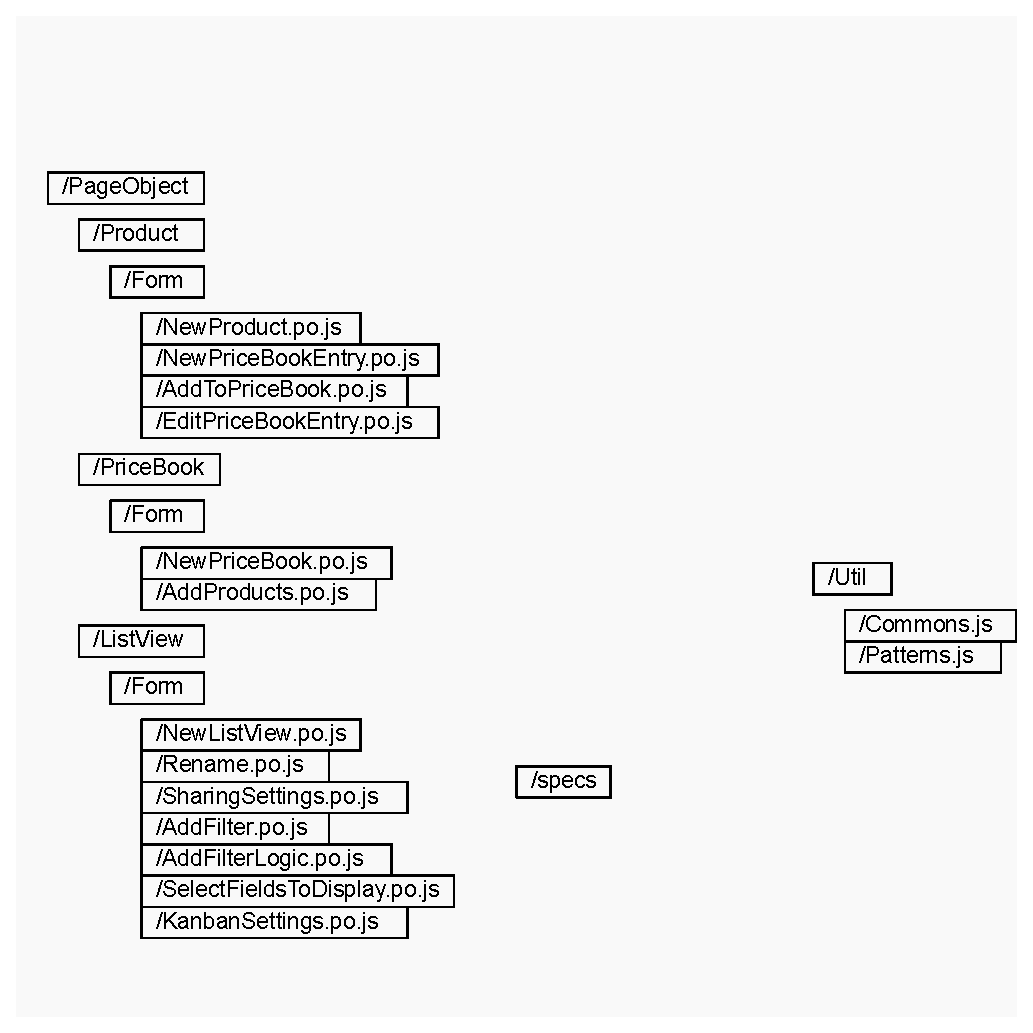
\includegraphics[width=1.0\textwidth]{graphics/diagram01.eps}
\caption{Diagrama de clases sobre las relaciones entre \emph{Page Objects}.}
\label{pom}
\source{Elaboración propia.}
\end{figure}

\section{\emph{Specs}}
Los \emph{Specs} representan las rutinas de automatización propiamente dichas,
cada \emph{spec} traduce directamente los pasos y comprobaciones que deberían
ser realizados en una ejecución de pruebas manual, de forma que la lectura de
cada rutina sea concisa y ordenada.

Un ejemplo de esto puede apreciarse en el caso de prueba \textbf{A001}, del cual
puede verse su especificación en el \emph{cuadro \ref{lltc}}, tal especificación
contiene la secuencia de pasos y el conjunto de verificaciones de la prueba como
se describen en el diagrama de secuencia de la \emph{figura \ref{sequence}}, y
estos a su vez traducidos a código fuente como se ve en la
\emph{figura \ref{spec}}.

\begin{table}
\renewcommand{\arraystretch}{1}
\linespread{1}
\centering
\begin{tabular}{|p{2.5cm}|p{2.8cm}|p{2.2cm}|p{2.8cm}|p{2.2cm}|}
\hline
\footnotesize{\textbf{Proyecto:}} &
\multicolumn{2}{c|}{\footnotesize{\emph{Salesforce} - Módulo de productos.}} &
\footnotesize{\textbf{Función:}} &
\multicolumn{1}{c|}{\footnotesize{[Nuevo]}} \\
\hline
\footnotesize{\textbf{ID:}} & \multicolumn{2}{c|}{\footnotesize{A001}} &
\footnotesize{\textbf{Prioridad:}} &
\multicolumn{1}{c|}{\footnotesize{Alta}} \\
\hline
\footnotesize{\textbf{Título:}} &
\multicolumn{4}{p{12.4cm}|}{\footnotesize{Producto es registrado con los valores
obligatorios establecidos después de accionado el botón «Guardar»}} \\
\hline
\footnotesize{\textbf{Descripción:}} &
\multicolumn{4}{p{12.4cm}|}{\footnotesize{Verificar que un nuevo producto sea
registrado correctamente cuando en el formulario de creación únicamente se han
establecido los valores obligatorios establecidos por este.}} \\
\hline
\multirow{2}{*}{\footnotesize{\textbf{Requerimientos:}}} &
\footnotesize{\textbf{Software:}} &
\multicolumn{3}{p{7.8cm}|}{\footnotesize{Navegador \emph{Google Chrome}
versión 70.0.3538.110}} \\
\cline{2-5}
& \footnotesize{\textbf{Instrucciones de inicialización:}} &
\multicolumn{3}{p{7.8cm}|}{\footnotesize{
\vspace{-3mm}
\begin{enumerate}
\item Autenticarse en la plataforma \emph{Salesforce}.
\item Clic en el «Iniciador de Aplicaciones».
\item Clic en el enlace «Productos».
\end{enumerate}
\vspace{-5mm}
}} \\
\hline
\footnotesize{\textbf{Pasos:}} &
\multicolumn{4}{p{11.8cm}|}{\footnotesize{
\vspace{-3mm}
\begin{enumerate}
\item Clic en el icono de «Controles de Vista de Lista».
\item Clic en el botón «Nuevo».
\item Rellenar el campo «Nombre del Producto» con el valor \textbf{TESTA001}.
\item Clic en el botón «Guardar».
\item Verificar que el mensaje enviado sea: \textbf{Producto TESTA001 ha sido creado}.
\item Verificar que en la vista de Producto el «Título» sea: \textbf{TESTA001}.
\item Verificar que en la vista de Producto el subtítulo «Código de Producto» este vació.
\item Verificar que en la vista de Producto el subtítulo «Familia de Producto» este vació.
\item Clic en el pestaña «Detalles».
\end{enumerate}
\vspace{-5mm}
}} \\
\hline
\multirow{2}{2.8cm}{\footnotesize{\textbf{Criterio de aceptación:}}} &
\footnotesize{\textbf{Resultado esperado:}} &
\multicolumn{3}{p{9.1cm}|}{\footnotesize{En la pestaña «Detalles», todos los
valores exceptuando el «Nombre de Producto» se encuentran con los valores
vacíos.}} \\
\cline{2-5}
& \footnotesize{\textbf{Verificación:}} &
\multicolumn{3}{p{9.1cm}|}{\footnotesize{Comprobar elemento por elemento que los
valores se encuentren vacíos, y que el campo «Nombre de Producto» sea igual a:
\textbf{TESTA001}.}} \\
\hline
\footnotesize{\textbf{Fecha:}} &
\multicolumn{1}{c|}{\footnotesize{2018-12-05}} &
\multicolumn{2}{l|}{\footnotesize{\textbf{Tiempo de ejecución:}}} &
\multicolumn{1}{c|}{\footnotesize{1 min 24 seg}} \\
\hline
\footnotesize{\textbf{Creado por:}} &
\multicolumn{4}{c|}{\footnotesize{CC - Carlos Caballero}} \\
\hline
\end{tabular}
\caption{Especificación del Caso de Prueba A001.}
\label{lltc}
\source{Elaboración propia.}
\end{table}

\begin{figure}
\centering
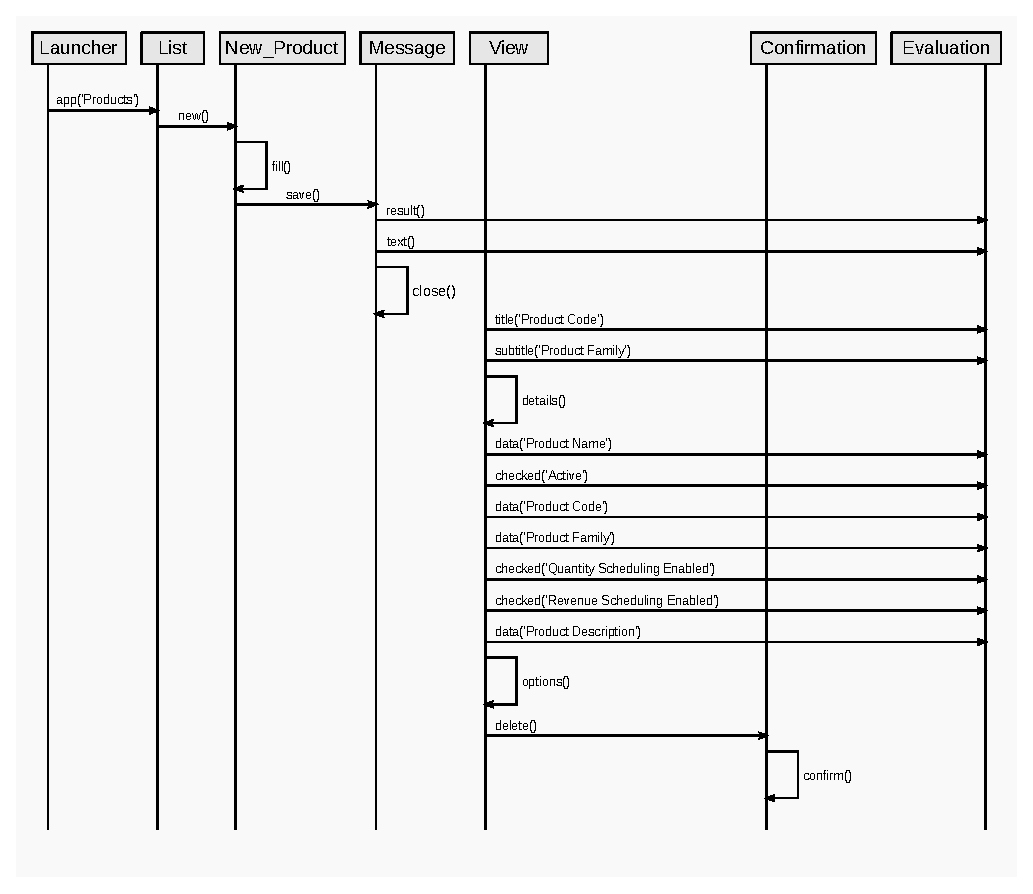
\includegraphics[width=1.0\textwidth]{graphics/diagram02.eps}
\caption{Diagrama de secuencia para el Caso de Prueba A001.}
\label{sequence}
\source{Elaboración propia.}
\end{figure}

\begin{figure}
\begin{verbatim}
it('A001 - Producto es registrado con los valores obligatorios '+
   'establecidos después de accionado el botón «Guardar»',()=>{
    let modal_new=Launcher.app('Products').new()
      , message=modal_new
            .fill({
                name:name
            })
            .save();

    expect(message.result()).to.equal('success');
    expect(message.text()).to.equal('Product "'+name+'" was created.');

    message.close();

    let view=new View();

    expect(view.title()).to.equal(name);
    expect(view.subtitle('Product Code')).to.equal('');
    expect(view.subtitle('Product Family')).to.equal('');

    view.details();

    expect(view.data('Product Name')).to.equal(name);
    expect(view.checked('Active')).to.equal(false);
    expect(view.data('Product Code')).to.equal('');
    expect(view.data('Product Family')).to.equal('');
    expect(view.checked('Quantity Scheduling Enabled')).to.equal(false);
    expect(view.checked('Revenue Scheduling Enabled')).to.equal(false);
    expect(view.data('Product Description')).to.equal('');

    view.options()
        .delete()
        .confirm();
});
\end{verbatim}
\caption{Automatización del Caso de Prueba A001.}
\label{spec}
\source{Elaboración propia.}
\end{figure}

\section{Ejecución de las pruebas}
Se realizó la ejecución de los casos de prueba automatizados contenidos en el
\emph{framework} en modo local, tal como se describe en el
\emph{\textbf{apéndice \ref{appendix_execution}}}.

En las \emph{figuras \ref{results-tests}} y \emph{\ref{results-type}}, se
condensan los resultados obtenidos de la ejecución de los casos de prueba, en
los cuales únicamente fallaron 2 casos de prueba, ambos relacionados a un mismo
formulario, como puede verse en el reporte de error adjunto, y debido al fallo
de estos también se bloquearon dos casos de prueba.

Presentados los resultados de la ejecución de las pruebas, vemos que de los 315
casos de prueba, únicamente existen 2 bloqueados, y dos fallidos. Por ende se
tiene 98.74\% de casos de prueba exitosos.

\begin{figure}
\centering
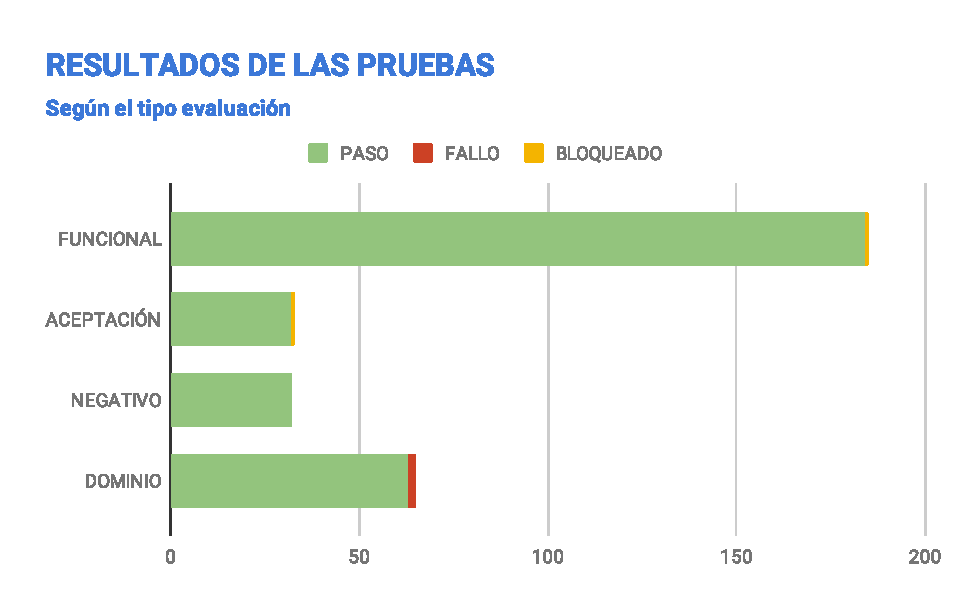
\includegraphics[width=1.0\textwidth]{graphics/results-tests.eps}
\caption{Resultados de las pruebas clasificadas por tipo de evaluación.}
\label{results-tests}
\source{Elaboración propia.}
\end{figure}

\begin{figure}
\centering
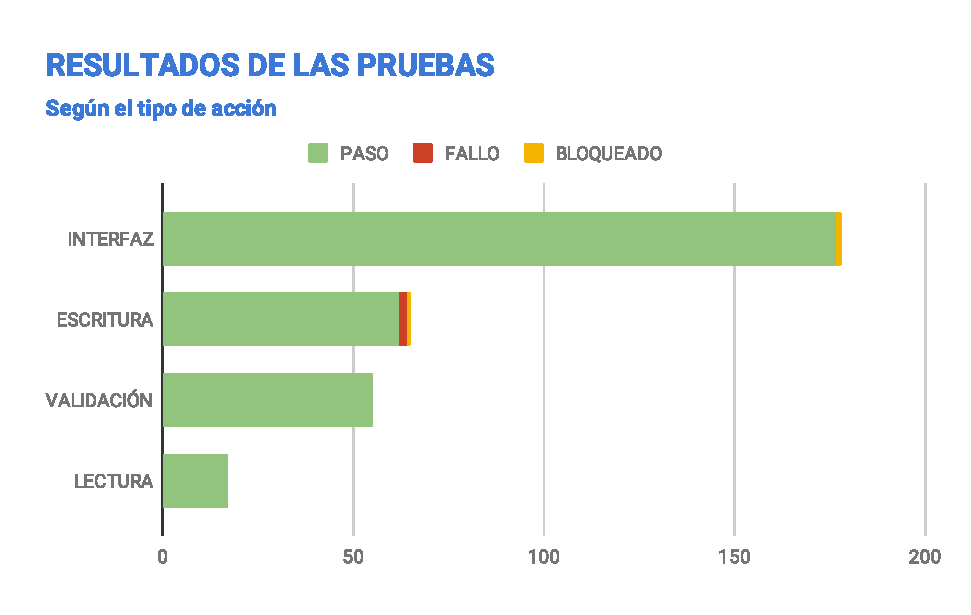
\includegraphics[width=1.0\textwidth]{graphics/results-type.eps}
\caption{Resultados de las pruebas clasificadas por tipo de acción a evaluar.}
\label{results-type}
\source{Elaboración propia.}
\end{figure}

\section{Reportes de Error}
Como anteriormente se mencionó, se encontraron cuatro casos de prueba no
exitosos, dos de ellos bloqueados, debido al fallo de otros dos casos de
prueba, es decir que no pueden verificarse apropiadamente, debido a que la
pre condición requerida es fallida, estos casos de prueba pueden verse en el
\emph{\textbf{apéndice \ref{appendix_bugreport}}}.

